\appendix
\setlength{\abovedisplayskip}{2pt}
\setlength{\belowdisplayskip}{2pt}

\section{Observation Model} \label{appdx:obs_model}
The observation model $\mathdutchcal{G}$ models how the objects $H_{1:K}$ cause the image observation $X \in \mathbbm{R}^{N \times M}$.
Here we provide a mechanistic justification for our choice of observation model by formulating the observation model as a probabilistic approximation to a deterministic rendering engine.

\textbf{Deterministic rendering engine:} Each object $H_k$ is rendered independently as the sub-image $I_k$ and the resulting $K$ sub-images are combined to form the final image observation $X$. To combine the sub-images, each pixel $I_{k(ij)}$ in each sub-image is assigned a depth $\delta_{k(ij)}$ that specifies the distance of object $k$ from the camera at coordinate $(ij)$. of the image plane. Thus the pixel $X_{(ij)}$ takes on the value of its corresponding pixel $I_{k(ij)}$ in the sub-image $I_k$ if object $k$ is closest to the camera than the other objects, such that
\footnotesize
\begin{equation}
    X_{(ij)} = \sum_{k=1}^K Z_{k(ij)} \cdot I_{k(ij)},
\end{equation}
\normalsize
where $Z_{k(ij)}$ is the indicator random variable $\mathbbm{1}[k = \argmin_{k \in K} \delta_{k(ij)}]$, allowing us to intuitively interpret $Z_{k}$ as segmentation masks and $I_{k}$ as color maps.

\textbf{Modeling uncertainty with the observation model:}
In reality we do not directly observe the depth values, so we must construct a probabilistic model to model our uncertainty:
\footnotesize
\begin{equation} \label{eqn:qppdx:obs_model}
    \mathdutchcal{G}\left(X| H_{1:K}\right) = \prod_{i,j=1}^{N,M} \sum_{k=1}^K m_{(ij)}(H_k) \cdot \mathdutchcal{g}\left(X_{(ij)} \sgiven H_k\right),
\end{equation}
\normalsize
where every pixel $(ij)$ is modeled through a set of mixture components \mbox{$\mathdutchcal{g}\left(X_{(ij)} \sgiven H_k\right) := p\left(X_{ij} | Z_{k(ij)}=1, H_k\right)$} that model how pixels of the individual sub-images $I_k$ are generated,
as well as through the mixture weights $m_{ij}(H_k):= p\left(Z_{k(ij)}=1| H_k\right)$ that model which point of each object is closest to the camera.

\section{Evidence Lower Bound}  \label{appdx:problem_formulation} \label{appdx:elbo}
Here we provide a derivation of the evidence lower bound. We begin with the log probability of the observations $X^{(1:T)}$ conditioned on a sequence of actions $a^{(0:T-1)}$:
\footnotesize
\begin{align}
    \log p\left(X^{(0:T)} \;\middle|\; a^{(0:T-1)}\right) &= \log \int_{h_{1:K}^{(0:T)}} p\left(X^{(0:T)}, h^{(0:T)}_{1:K} \;\middle|\; a^{(0:T-1)}\right) \; dh_{1:K}^{(0:T)}.\nonumber\\
    &= \log \int_{h_{1:K}^{(0:T)}} p\left(X^{(0:T)}, h^{(0:T)}_{1:K} \;\middle|\; a^{(0:T-1)}\right) \frac{q\left(h^{(0:T)}_{1:K} \given \cdot \right)}{q\left(h^{(0:T)}_{1:K} \given \cdot \right)} \; dh_{1:K}^{(0:T)}.\nonumber\\
    &= \log \mathbb{E}_{h^{(0:T)}_{1:K} \sim q\left(H^{(0:T)}_{1:K} \given \cdot \right)} \left[\frac{p\left(X^{(0:T)}, h^{(0:T)}_{1:K} \;\middle|\; a^{(0:T-1)}\right)}{q\left(h^{(0:T)}_{1:K} \given \cdot \right)}\right]\nonumber\\
    &\geq \mathbb{E}_{h^{(0:T)}_{1:K} \sim q\left(H^{(0:T)}_{1:K} \given \cdot \right)} \log \left[\frac{p\left(X^{(0:T)}, h^{(0:T)}_{1:K} \;\middle|\; a^{(0:T-1)}\right)}{q\left(h^{(0:T)}_{1:K} \given \cdot \right)}\right]. \label{eqn:appdx:elbo}
\end{align}
\normalsize
We have freedom to choose the approximating distribution $q\left(H^{(0:T)}_{1:K} \given \cdot \right)$ so we choose it to be conditioned on the past states and actions, factorized across time:
\footnotesize
\begin{equation*}
    q\left(H^{(0:T)}_{1:K} \given x^{(0:T)}, a^{(0:T)}\right) = q\left(H^{(0)}_{1:K} \sgiven x^{(0)}\right) \prod_{t=1}^T q\left(H^{(t)}_{1:K} \given H^{(t-1)}_{1:K}, x^{(t)}, a^{(t-1)}\right)
\end{equation*}
\normalsize
With this factorization, we can use linearity of expectation to decouple Equation~\ref{eqn:appdx:elbo} across timesteps:
\footnotesize
\begin{equation*}
    \mathbb{E}_{h^{(0:T)}_{1:K} \sim q\left(H^{(0:T)}_{1:K} \sgiven x^{(0:T)}, a^{(0:T)}\right)} \log \left[\frac{p\left(X^{(0:T)}, h^{(0:T)}_{1:K} \;\middle|\; a^{(0:T-1)}\right)}{q\left(h^{(0:T)}_{1:K} \sgiven x^{(0:T)}, a^{(0:T)}\right)}\right] = \sum_{t=0}^{(t)} \mathcal{L}^{(t)}_{\text{r}} - \mathcal{L}^{(t)}_{\text{c}},
\end{equation*}
\normalsize
where at the first timestep
\footnotesize
\begin{align*}
    \mathcal{L}^{(0)}_{\text{r}} &= \mathbb{E}_{h_{1:K}^{(0)} \sim q\left(H_{1:K}^{(0)} \given X^{(0)}\right)}\left[ \log p\left(X^{(0)} \given h_{1:K}^{(0)} \right)\right]\\
     \mathcal{L}^{(0)}_{\text{c}} &= D_{KL}\left(q\left(H_{1:K}^{(0)} \given X^{(0)}\right) \kld p\left(H_{1:K}^{(0)}\right)\right)
\end{align*}
\normalsize
and at subsequent timesteps
\footnotesize
\begin{align*}
    \mathcal{L}^{(t)}_{\text{r}} &= \mathbb{E}_{h^{(t)}_{1:K} \sim q\left(H^{(t)}_{1:K} \sgiven h^{(0:t-1)}_{1:K}, X^{(0:t)}, a^{(0:t-1)} \right)}\left[\log p\left(X^{(t)} \given h^{(t)}_{1:K}\right)\right]\\
    \mathcal{L}^{(t)}_{\text{c}} &= \mathbb{E}_{h^{(t-1)}_{1:K} \sim q\left(H^{(t-1)}_{1:K} \sgiven h^{(0:t-2)}_{1:K}, X^{(1:t-1)}, a^{(0:t-2)} \right)}\left[D_{KL}\left(q\left(H^{(t)}_{1:K} \given h^{(t-1)}_{1:K}, X^{(t)}, a^{(t-1)}\right) \kld p\left(H^{(t)}_{1:K} \given h^{(t-1)}_{1:K}, a^{(t-1)} \right)\right)\right].
\end{align*}
\normalsize
By the Markov property, the marginal $q(H^{(t)}_{1:K} \sgiven h^{(0:t-1)}_{1:K}, X^{(0:t)}, a^{(0:t-1)})$ is computed recursively as
\footnotesize
\begin{equation*}
    \mathbb{E}_{h^{(t-1)} \sim q\left(H^{(t-1)}_{1:K} \sgiven h^{(0:t-2)}_{1:K}, X^{(0:t-1)}, a^{(0:t-2)} \right)}\left[ q\left(H^{(t)}_{1:K} \given h^{(t-1)}_{1:K}, X^{(t)}, a^{(t-1)} \right) \right]
\end{equation*}
\normalsize
whose base case is $q\left(H^{(0)} \,|\, X^{(0)} \right)$ when $t=0$. 

We approximate observation distribution $p(X \sgiven H_{1:K})$ and the dynamics distribution $p(H'_{1:K} \sgiven H_{1:K}, a)$ by learning the parameters of the observation model $\mathdutchcal{G}$ and dynamics model $\mathdutchcal{D}$ respectively as outputs of neural networks.
We approximate the recognition distribution $q(H^{(t)}_{1:K} \sgiven h^{(t-1)}_{1:K}, X^{(t)}, a^{(t-1)})$ via an inference procedure that refines better estimates of the posterior parameters, computed as an output of a neural network.
To compute the expectation in the marginal $q(H^{(t)}_{1:K} \sgiven h^{(0:t-1)}_{1:K}, X^{(0:t)}, a^{(0:t-1)})$, we follow standard practice in amortized variational inference by approximating the expectation with a single sample of the sequence $h^{(0:t-1)}_{1:K}$ by sequentially sampling the latents for one timestep given latents from the previous timestep, and optimizing the ELBO via stochastic gradient ascent~\citep{doersch2016tutorial,kingma2013auto,rezende2014stochastic}.

\section{Posterior Predictive Distribution}
\label{appdx:posterior_predictive_distribution}
Here we provide a derivation of the posterior predictive distribution for the dynamic latent variable model with multiple latent states.
Section~\ref{appdx:elbo} described how we compute the distributions $p(X \sgiven H_{1:K})$, $p(H'_{1:K} \sgiven H_{1:K}, a)$, $q(H^{(t)}_{1:K} \sgiven h^{(t-1)}_{1:K}, X^{(t)}, a^{(t-1)})$, and $q(H_{1:K}^{(0:T)} \sgiven x^{(1:T)}, a^{(1:T)})$.
Here we show that these distributions can be used to approximate the predictive posterior distribution $p(X^{(T+1:T+d)} \sgiven x^{(0:T)}, a^{(0:T+d)})$ by maximizing the following lower bound:
\footnotesize
\begin{align}
    \log p\left(X^{(T+1:T+d)} \given x^{(0:T)}, a^{(0:T+d)}\right) &=\int_{h_{1:K}^{(0:T+d)}} p\left(X^{(T+1:T+d)}, h_{1:K}^{(0:T+d)} \given x^{(0:T)}, a^{(0:T+d)}\right) \;dh_{1:K}^{(0:T+d)}\nonumber\\
    &=\int_{h_{1:K}^{(0:T+d)}} p\left(X^{(T+1:T+d)}, h_{1:K}^{(0:T+d)} \given x^{(0:T)}, a^{(0:T+d)}\right) \frac{q\left(h_{1:K}^{(0:T+d)} \given \cdot \right)}{q\left(h_{1:K}^{(0:T+d)} \given \cdot \right)}\;dh_{1:K}^{(0:T+d)}\nonumber\\
    &=\log \mathbb{E}_{h_{1:K}^{(0:T+d)} \sim q\left(H_{1:K}^{(0:T+d)} \given \cdot \right)} \left[\frac{p\left(X^{(T+1:T+d)}, h_{1:K}^{(0:T+d)} \given x^{(0:T)}, a^{(0:T+d)}\right)}{q\left(h_{1:K}^{(0:T+d)} \given \cdot \right)}\right]\nonumber\\
    &\geq \mathbb{E}_{h_{1:K}^{(0:T+d)} \sim q\left(H_{1:K}^{(0:T+d)} \given \cdot \right)} \log \left[\frac{p\left(X^{(T+1:T+d)}, h_{1:K}^{(0:T+d)} \given x^{(0:T)}, a^{(0:T+d)}\right)}{q\left(h_{1:K}^{(0:T+d)} \given \cdot \right)}\right].\label{eqn:appdx:post_pred_elbo}
\end{align}
\normalsize
The numerator $p(X^{(T+1:T+d)}, h_{1:K}^{(0:T+d)} \sgiven x^{(0:T)}, a^{(0:T+d)})$ can be decomposed into two terms, one of which involving the posterior $p(h_{1:K}^{(0:T+d)} \sgiven x^{(0:T)}, a^{(0:T+d)})$:
\footnotesize
\begin{equation*}
    p\left(X^{(T+1:T+d)}, h_{1:K}^{(0:T+d)} \given x^{(0:T)}, a^{(0:T+d)}\right) = p\left(X^{(T+1:T+d)} \given h_{1:K}^{(0:T+d)}\right) p\left(h_{1:K}^{(0:T+d)} \given x^{(0:T)}, a^{(0:T+d)}\right),
\end{equation*}
\normalsize
This allows Equation~\ref{eqn:appdx:post_pred_elbo} to be broken up into two terms:
\footnotesize
\begin{align*}
    \mathbb{E}_{h_{1:K}^{(0:T+d)} \sim q\left(H_{1:K}^{(0:T+d)} \given \cdot \right)} \log p\left(X^{(T+1:T+d)} \given h_{1:K}^{(0:T+d)}\right) -D_{KL}\left(q\left(H_{1:K}^{(0:T+d)} \given \cdot \right) \kld p\left(H_{1:K}^{(0:T+d)} \given x^{(0:T)}, a^{(0:T+d)}\right) \right)
\end{align*}
\normalsize
Maximizing the second term, the negative KL-divergence between the variational distribution $q(H_{1:K}^{(0:T+d)} \sgiven \cdot)$ and the posterior $p(H_{1:K}^{(0:T+d)} \sgiven x^{(0:T)}, a^{(0:T+d)})$ is the same as maximizing the following lower bound:
\footnotesize
\begin{equation} \label{eqn:appdx:neg_kl}
    \mathbb{E}_{h_{1:K}^{(0:T)} \sim q\left(h_{1:K}^{(0:T)} \given \cdot \right)} \log p\left(x^{(0:T)} \given h_{1:K}^{(0:T)}, a^{(0:T-1)}\right) - D_{KL}\left(q\left(H_{1:K}^{(0:T+d)} \given \cdot \right) \kld p\left(H_{1:K}^{(0:T+d)} \given a^{(0:T+d)}\right) \right)
\end{equation}
\normalsize
where the first term is due to the conditional independence between $X^{(0:T)}$ and the future states $H_{1:K}^{(T+1:T+d)}$ and actions $A^{(T+1:T+d)}$.
% Note that Equation~\ref{eqn:appdx:neg_kl} is not the same as the ELBO in Equation~\ref{eqn:appdx:elbo} because the KL divergence term is with respect to distributions over $H_{1:K}^{(0:T+d)}$, not $H_{1:K}^{(0:T)}$.
We choose to express $q\left(H_{1:K}^{(0:T+d)} \given \cdot \right)$ as conditioned on past states and actions, factorized across time:
\footnotesize
\begin{equation*}
    q\left(H^{(0:T+d)} \given x^{(0:T)}, a^{(0:T+d-1)}\right) = q\left(H^{(0)}_{1:K} \sgiven x^{(0)}\right) \prod_{t=1}^{T+d} q\left(H^{(t)}_{1:K} \given H^{(t-1)}_{1:K}, x^{(t)}, a^{(t-1)}\right).
\end{equation*}
\normalsize
In summary, Equation~\ref{eqn:appdx:post_pred_elbo} can be expressed as
\footnotesize
\begin{align*}
    &\mathbb{E}_{h_{1:K}^{(0:T+d)} \sim q\left(H^{(0:T+d)} \given x^{(0:T)}, a^{(0:T+d-1)}\right)} \log p\left(X^{(T+1:T+d)} \given h_{1:K}^{(0:T+d)}\right)\\
    + &\mathbb{E}_{h_{1:K}^{(0:T)} \sim q\left(H^{(0:T)} \given x^{(0:T)}, a^{(0:T-1)}\right)} \log p\left(x^{(0:T)} \given h_{1:K}^{(0:T)}, a^{(0:T-1)}\right) \\
    - &D_{KL}\left(q\left(H^{(0:T+d)} \given x^{(0:T)}, a^{(0:T+d-1)}\right) \kld p\left(H_{1:K}^{(0:T+d)} \given a^{(0:T+d)}\right) \right)
\end{align*}
\normalsize
which can be interpreted as the standard ELBO objective for timesteps $0:T$, plus an addition reconstruction term for timesteps $T+1:T+d$, a reconstruction term for timesteps $0:T$.
We can maximize this using the same techniques as maximizing Equation~\ref{eqn:appdx:elbo}.

Whereas approximating the ELBO in Equation~\ref{eqn:appdx:post_pred_elbo} can be implemented by rolling out OP3 to predict the next observation via teacher forcing~\citep{williams1989learning}, approximating the posterior predictive distribution in Equation~\ref{eqn:appdx:post_pred_elbo} can be implemented by rolling out the dynamics model $d$ steps beyond the last observation and using the observation model to predict the future observations.


\section{Interactive Inference} \label{appdx:interactive_inference}
Algorithms~\ref{alg:appdx:timestep_0} and~\ref{alg:appdx:timestep_t} detail $M$ steps of the interactive inference algorithm at timestep $0$ and $t \in [1, T]$ respectively.
Algorithm~\ref{alg:appdx:timestep_0} is equivalent to the IODINE algorithm described in~\citep{greff2019iodine}.
Recalling that $\lambda_{1:K}$ are the parameters for the distribution of the random variables $H_{1:K}$, we consider in this paper the case where this distribution is an isotropic Gaussian (e.g. $\mathcal{N}(\lambda_k)$ where $\lambda_k = (\mu_k, \sigma_k)$), although OP3 need not be restricted to the Gaussian distribution.
The \textit{refinement network} $f_{\mathdutchcal{q}}$ produces the parameters for the distribution $\mathdutchcal{q}(H^{(t)}_{k} \sgiven h^{(t-1)}_{k}, x^{(t)}, a^{(t)})$.
The \textit{dynamics network} $f_{\mathdutchcal{d}}$ produces the parameters for the distribution $\mathdutchcal{d}(H^{(t)}_k \sgiven h^{(t-1)}_k, h^{(t-1)}_{[\neq k]}, a^{(t)})$.
To implement $\mathdutchcal{q}$, we repurpose the dynamics model to transform $h_k^{(t-1)}$ into the initial posterior estimate $\lambda_k^{(0)}$ and then use $f_{\mathdutchcal{q}}$ to iteratively update this parameter estimate.
$\beta_k$ indicates the auxiliary inputs into the refinement network used in~\citep{greff2019iodine}.
We mark the major areas where the algorithm at timestep $t$ differs from the algorithm at timestep $0$ in \textcolor{NavyBlue}{blue}.

\begin{algorithm}[H]
    \caption{Interactive Inference: Timestep $0$}
    \label{alg:appdx:timestep_0}
    \footnotesize
    \begin{algorithmic}[1]
        \State \textbf{Input:} observation $x^{(0)}$
        \State \textbf{Initialize:} parameters $\lambda^{(0,0)}$
        \For{$i = 0$ \textbf{to} $M-1$}
            \State Sample $h^{(0,i)}_k \sim \mathcal{N}\left(\lambda^{(0,i)}_k\right)$ for each entity $k$
            \State Evaluate $\mathcal{L}^{(0,i)} \approx \log \mathdutchcal{G}\left(x^{(0)} \,|\, h^{(0,i)}_{1:K} \right) - D_{KL}\left(\mathcal{N}\left(\lambda_{1:K}^{(0,i)}\right) \kld \mathcal{N}\left(0, I\right)\right)$ 
            \State Calculate $\nabla_{\lambda_k} \mathcal{L}^{(0, i)}$ for each entity $k$
            \State Assemble auxiliary inputs $\beta_k$ for each entity $k$
            \State Update $\lambda^{(0, i+1)}_k \gets f_{\text{refine}} \left(x^{(0)}, \nabla_\lambda \mathcal{L}^{(0, i)}, \lambda^{(0, i)}, \beta_k^{(0,i)}\right)$ for each entity $k$
        \EndFor
        \State \Return $\lambda^{(0, M)}$
    \end{algorithmic}
\end{algorithm}

\begin{algorithm}[H]
    \caption{Interactive Inference: Timestep $t$}
    \label{alg:appdx:timestep_t}
    \footnotesize
    \begin{algorithmic}[1] 
        \State \textbf{Input:} observation $x^{(t)}$, \textcolor{NavyBlue}{previous action $a^{(t-1)}$, previous entity states $h^{(t-1)}_{1:K}$}
        \State \textcolor{NavyBlue}{\textbf{Predict} $\lambda^{(t,0)}_k \gets f_{\mathdutchcal{d}}\left(h^{(t-1)}_k, h^{(t-1)}_{[\neq k]}, a^{(t-1)}\right)$} for each entity $k$
        \For{$i = 0$ \textbf{to} $M-1$}
            \State Sample $h_k^{(t,i)} \sim \mathcal{N}\left(\lambda^{(t, i)}\right)$ for each entity $k$
            \State Evaluate $\mathdutchcal{L}^{(t, i)} \approx \log \mathdutchcal{G}\left(x^{(t)} \,|\, h_{1:K}^{(t)} \right) - D_{KL}\left({\mathcal{N}\left(\lambda^{(t,i)}_{1:K}\right) \kld \textcolor{NavyBlue}{\mathcal{N}\left(\lambda^{(t,0)}_{1:K}\right)}}\right)$
            \State Calculate $\nabla_{\lambda_k} \mathdutchcal{L}^{(t, i)}$ for each entity $k$
            \State Assemble auxiliary inputs $\beta_k$ for each entity $k$
            \State Update $\lambda^{(t, i+1)}_k \gets f_{\mathdutchcal{q}}\left(x^{(t)}, \nabla_{\lambda_k} \mathdutchcal{L}^{(t, i)}, \lambda^{(t, i)}_k, \beta_k^{(t,i)}\right)$ for each entity $k$
        \EndFor
        \State \Return $\lambda^{(t, M)}$
    \end{algorithmic}
\end{algorithm}

\paragraph{Training:} We can train the entire OP3 system end-to-end by backpropagating through the entire inference procedure, using the ELBO at every timestep as a training signal for the parameters of $\mathcal{G}$, $\mathcal{D}$, $\mathcal{Q}$ in a similar manner as~\citep{van2018relational}.
However, the interactive inference algorithm can also be naturally be adapted to predict rollouts by using the dynamics model to propagate the $\lambda_{1:K}$ for multiple steps, rather than just the one step for predicting $\lambda_{1:K}^{(t,0)}$ in line 2 of Algorithm~\ref{alg:appdx:timestep_t}.
To train OP3 to rollout the dynamics model for longer timescales, we use a curriculum that increases the prediction horizon throughout training.

\section{Cost Function}
Let $\hat{I}(H_{k}) := m(H_k) \cdot \mathdutchcal{g}\left(X \sgiven H_k\right)$ be a \textit{masked} sub-image (see Appdx:~\ref{appdx:obs_model}).
We decompose the cost of a particular configuration of objects into a distance function between entity states, $\mathdutchcal{c}(H_a, H_b)$. For the first environment with single-step planning we use $L_2$ distance of the corresponding masked subimages: $\mathdutchcal{c}(H_a, H_b) = L_2(\hat{I}(H_a), \hat{I}(H_b))$.
For the second environment with multi-step planning we a different distance function since the previous one may care more about if a shape matches than if the color matches. We instead use a form of intersection over union but that counts intersection if the mask aligns and pixel color values are close $\mathdutchcal{c}(H_a, H_b) = 1 -  \frac{{\sum_{i,j} m_{ij}(H_a) > 0.01 \text{ and } m_{ij}(H_b) > 0.01} \text{ and } L_2(\mathdutchcal{g}(H_a)_{(ij)}, \mathdutchcal{g}(H_b)_{(ij)}) < 0.1}{\sum_{i,j} m_{ij}(H_a) > 0.01 \text{ or } m_{ij}(H_b) > 0.01}$. We found this version to work better since it will not give low cost to moving a wrong color block to the position of a different color goal block.

\section{Architecture and Hyperparameter Details} \label{appdx:arch_details}
We use similar model architectures as in \citep{greff2019iodine} and so have rewritten some details from their appendix here. Differences include the dynamics model, inclusion of actions, and training procedure over sequences of data.  
Like~\citep{hafner2018learning}, we define our latent distribution of size $R$ to be divided into a deterministic component of size $R_d$ and stochastic component of size $R_s$.
We found that splitting the latent state into a deterministic and stochastic component (as opposed to having a fully stocahstic representation) was helpful for convergence.
We parameterize the distribution of each $H_k$ as a diagonal Gaussian, so the output of the refinement and dynamics networks are the parameteres of a diagonal Gaussian.
We parameterize the output of the observation model also as a diagonal Gaussian with means $\mu$ and global scale $\sigma=0.1$. The observation network outputs the $\mu$ and mask $m_k$.

\textbf{Training:} All models are trained with the ADAM optimizer \citep{kingma2014adam} with default parameters and a learning rate of 0.0003. We use gradient clipping as in \citep{Pascanu2012UnderstandingTE} where if the norm of global gradient exceeds 5.0 then the gradient is scaled down to that norm. 

\textbf{Inputs:} 
For all models, we use the following inputs to the refinement network, where LN means Layernorm and SG means stop gradients.
The following image-sized inputs are concatenated and fed to the corresponding convolutional network: 

\begin{center}
\begin{tabular}{llccc}
\toprule
    Description & Formula & LN & SG & Ch.\\ \midrule
    image & $X$ & & & 3 \\
    means & $\mu$ &  & & 3  \\
    mask  & $m_k$ & & & 1 \\
    mask-logits & $\hat{m}_k$ & & & 1 \\
    mask posterior & $p(m_k|X,\mu)$ & & & 1 \\
    gradient of means & $\nabla_{μ_k}\mathcal{L}$ & \checkmark & \checkmark & 3 \\
    gradient of mask & $\nabla_{m_k}\mathcal{L}$ & \checkmark & \checkmark & 1 \\
    pixelwise likelihood & $p(X \sgiven H)$ & \checkmark & \checkmark & 1 \\
    leave-one-out likelih. & $p(X \sgiven H_{i \neq k})$ & \checkmark & \checkmark & 1 \\
    coordinate channels & & & & 2 \\
    \midrule
    \multicolumn{4}{r}{total:} & 17 \\
    \bottomrule
\end{tabular}
\end{center}

\subsection{Observation and Refinement Networks}
The posterior parameters $\lambda_{1:K}$ and their gradients are flat vectors, and we concatenate them with the output of the convolutional part of the refinement network and use the result as input to the refinement LSTM:

\begin{center}
\begin{tabular}{llcc}
\toprule
    Description & Formula & LN & SG\\ \midrule
    gradient of posterior & $\nabla_{\lambda_k}\mathcal{L}$ & \checkmark & \checkmark \\
    posterior & $\lambda_k$ & &\\
    \bottomrule
\end{tabular}
\end{center}

All models use the ELU activation function and the convolutional layers use a stride equal to 1 and padding equal to 2 unless otherwise noted. For the table below $R_s=64$ and $R=128$.

\begin{center}
\begin{tabular}{lccl}
    \multicolumn{4}{c}{\textbf{Observation Model Decoder}}\\ 
    \toprule
    Type & Size/\textit{Ch.} & Act. Func. & Comment\\ \midrule
    Input: $H_i$  & $R$ &  & \\
    Broadcast & \textit{$R$+2} & & + coordinates\\
    Conv $5\times5$ & \textit{32} & ELU & \\
    Conv $5\times5$ & \textit{32} & ELU & \\
    Conv $5\times5$ & \textit{32} & ELU & \\
    Conv $5\times5$ & \textit{32} & ELU & \\
    Conv $5\times5$ & \textit{4} & Linear  & RGB + Mask\\
    \bottomrule
\end{tabular}
\end{center}

\begin{center}
\begin{tabular}{lccl}
    \multicolumn{4}{c}{\textbf{Refinement Network}}\\
    \toprule
    Type & Size/\textit{Ch.} & Act. Func. & Comment\\ \midrule
    MLP & 128 & Linear & \\
    LSTM & 128 & Tanh & \\
    Concat $[{\lambda_i}, \nabla_{\lambda_i}]$ & $2R_s$ & & \\
    MLP & 128 & ELU & \\
    Avg. Pool & $R_s$ & \\
    Conv $3\times3$ & \textit{$R_s$}  & ELU & \\
    Conv $3\times3$ & \textit{32}  & ELU & \\
    Conv $3\times3$ & \textit{32}  & ELU & \\
    Inputs & \textit{17}  & & \\
    \bottomrule
\end{tabular}
\end{center}

\subsection{Dynamics Model} \label{appdx:dyn_model}
The dynamics model $\mathcal{D}$ models how each entity $H_k$ is affected by action $A$ and the other entity $H_{[\neq k]}$.
It applies the same function $\mathdutchcal{d}(H_k' \sgiven H_k, H_{[\neq k]}, A)$ to each state, composed of several functions illustrated and described in Fig.~\ref{fig:dynamics}:
\begin{footnotesize}
\begin{align*}
&\tilde{H}_k = d_{o}(H_k) \qquad
\tilde{A} = d_{a}(A^t) \qquad
\tilde{H}_k^{\text{act}} = d_{ao}(\tilde{H}_k \tilde{A}) \\
&H_k^{\text{interact}} = \sum_{i \neq k}^K d_{oo}(\tilde{H_i}^{\text{act}}, \tilde{H_k}^{\text{act}}) \qquad
H_{k}^{'} = d_{\text{comb}}(\tilde{H}_k^{\text{act}}, H_k^{\text{interact}}),
\end{align*}
\end{footnotesize}
where for a given entity $k$, $d_{ao}(\tilde{H}_k \tilde{A}) := d_{\text{act-eff}}(\tilde{H}_k, \tilde{A}) \cdot d_{\text{act-att}}(\tilde{H}_k, \tilde{A})$ computes how $(d_{\text{act-eff}})$ and to what degree $(d_{\text{act-att}})$ an action affects the entity and $d_{oo}(\tilde{H_i}^{\text{act}}, \tilde{H_k}^{\text{act}}) := d_{\text{obj-eff}}(\tilde{H}_i^{\text{act}}, \tilde{H}_k^{\text{act}}) \cdot d_{\text{obj-att}}(\tilde{H}_i^{\text{act}}, \tilde{H}_k^{\text{act}}
)$ computes how $(f_{\text{obj-eff}})$ and to what degree $(d_{\text{obj-att}})$ other entities affect that entity.
$d_{\text{obj-eff}}$ and $d_{\text{obj-att}}$ are shared across all entity pairs. The other functions are shared across all entities. The dynamics network takes in a sampled state and outputs the parameters of the posterior distribution. Similar to~\citep{hafner2018learning} the output $H'_k$ is then split into deterministic and stochastic components each of size 64 with separate networks $f_{\text{det}}$ and $f_{\text{sto}}$. All functions are parametrized by single layer MLPs.

\begin{center}
\begin{tabular}{lccl}
    \multicolumn{4}{c}{\textbf{Dynamics Network}}\\
    \toprule
    Function  & Output & Act. Func. & MLP Size\\ \midrule
    $d_o(H_k$) & $\tilde{H_k}$ & ELU & 128 \\
    $d_a(A)$ & $\tilde{A}$ & ELU &  32 \\
    $d_{\text{act-eff}}(\tilde{H_k}, \tilde{A})$ &  & ELU & 128 \\
    $d_{\text{act-att}}(\tilde{H_k}, \tilde{A})$ &  & Sigmoid & 128 \\
    $d_{\text{obj-eff}}(\tilde{H}_i^{\text{act}}, \tilde{H}_j^{\text{act}})$ &  & ELU & 256 \\
    $d_{\text{obj-att}}(\tilde{H}_i^{\text{act}}, \tilde{H}_k^{\text{act}})$ &  & Sigmoid & 256 \\
    $d_{\text{comb}}(\tilde{H}_i^{\text{act}}, \tilde{H}_k^{\text{interact}})$ &  $H'_k$& ELU & 256 \\
    $f_{\text{det}}(H'_k)$ &  $H'_{\text{k,det}}$&  & 128 \\
    $f_{\text{sto}}(H'_k)$ &  $H'_{\text{k,sto}}$&  & 128 \\
    \bottomrule
\end{tabular}
\end{center}

This architectural choice for the dynamics model is an action-conditioned modification of the interaction function used in Relational Neural Expectation Maximization (RNEM)~\citep{van2018relational}, which is a latent-space attention-based modification of the Neural Physics Engine (NPE)~\citep{chang2016compositional}, which is one of a broader class of architectures known as graph networks~\citep{battaglia2018relational}.


\section{Experiment Details}

\subsection{Single-Step Block-Stacking}
The training dataset has 60,000 trajectories each containing before and after images of size 64x64 from \cite{janner2018reasoning}. Before images are constructed with actions which consist of choosing a shape (cube, rectangle, pyramid), color, and an $(x, y, z)$ position and orientation for the block to be dropped. At each time step, a block is dropped and the simulation runs until the block settles into a stable position. The model takes in an image containing the block to be dropped and must predict the steady-state effect. Models were trained on scenes with 1 to 5 blocks with $K = 7$ entity variables. The cross entorpy method (CEM) begins from a uniform distribution on the first iteration, uses a population size of 1000 samples per iteration, and uses 10\% of the best samples to fit a Gaussian distribution for each successive iteration.

\begin{figure}[h!]
    \centering
    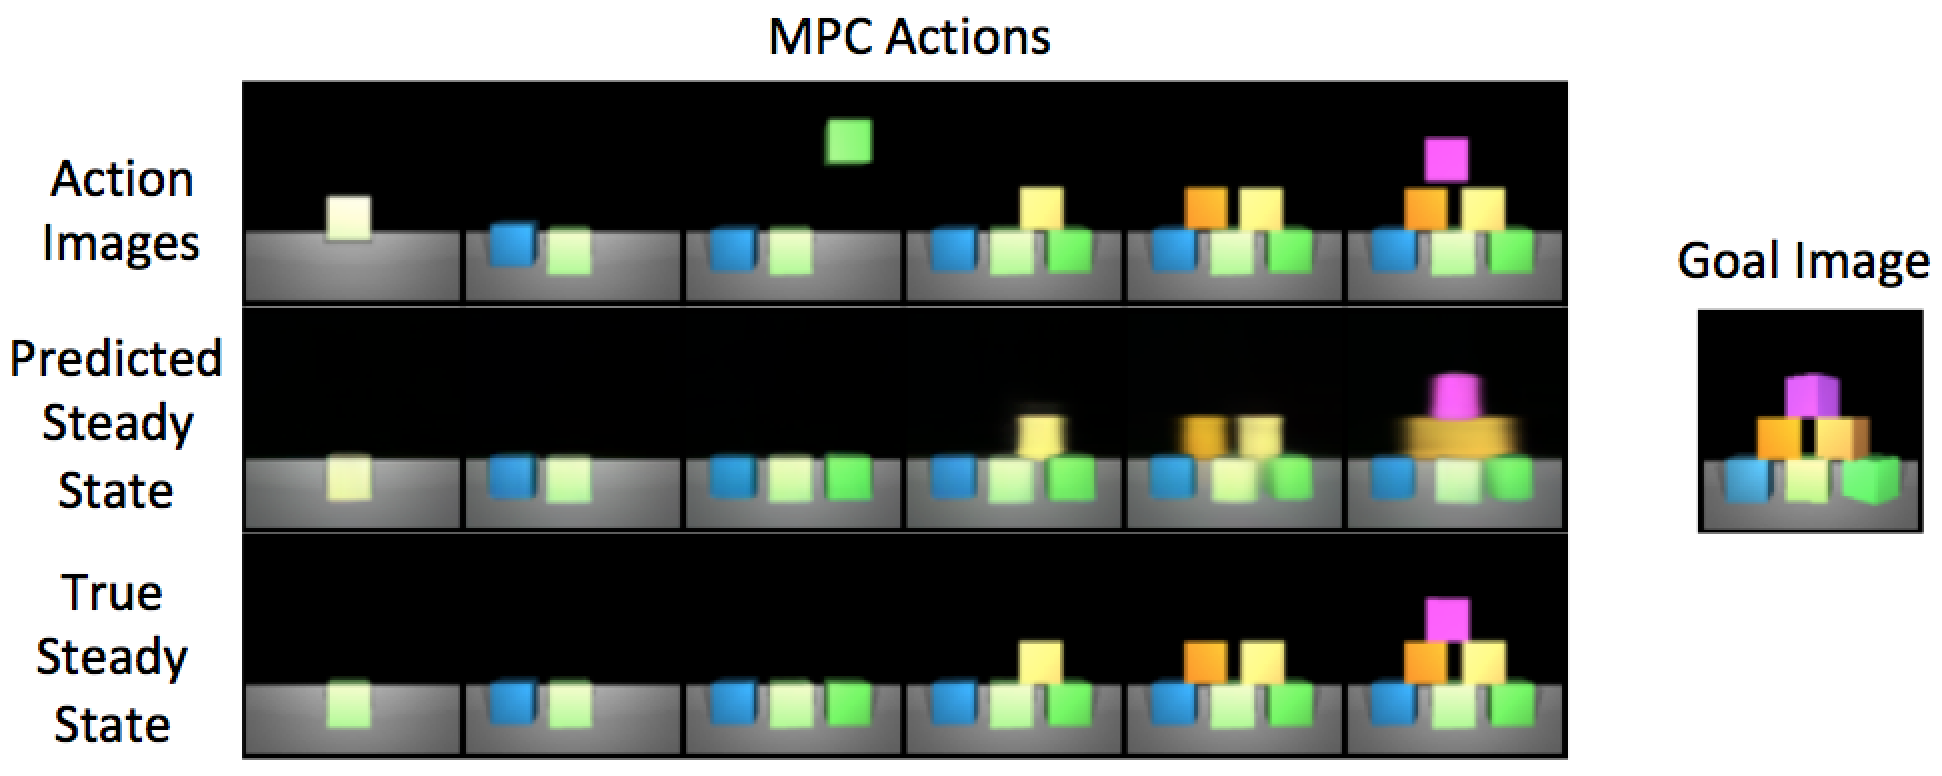
\includegraphics[width=1\columnwidth]{figs/experiments/mpc_labeled_long.png}
    \caption{Qualitative results on building a structure from the dataset in~\citep{janner2018reasoning}. The input is an "action image," which depicts how an action intervenes on the state by raising a block in the air. OP3 is trained to predict the steady-state outcome of dropping the block. We see how OP3 is able to accurately and consistently predict the steady state effect, successively capturing the effect of inertial dynamics (gravity) and interactions with other objects.}   \label{fig:mpc_results}
\end{figure}

\begin{figure}[t]
    \centering
    \hspace{-4pt}
    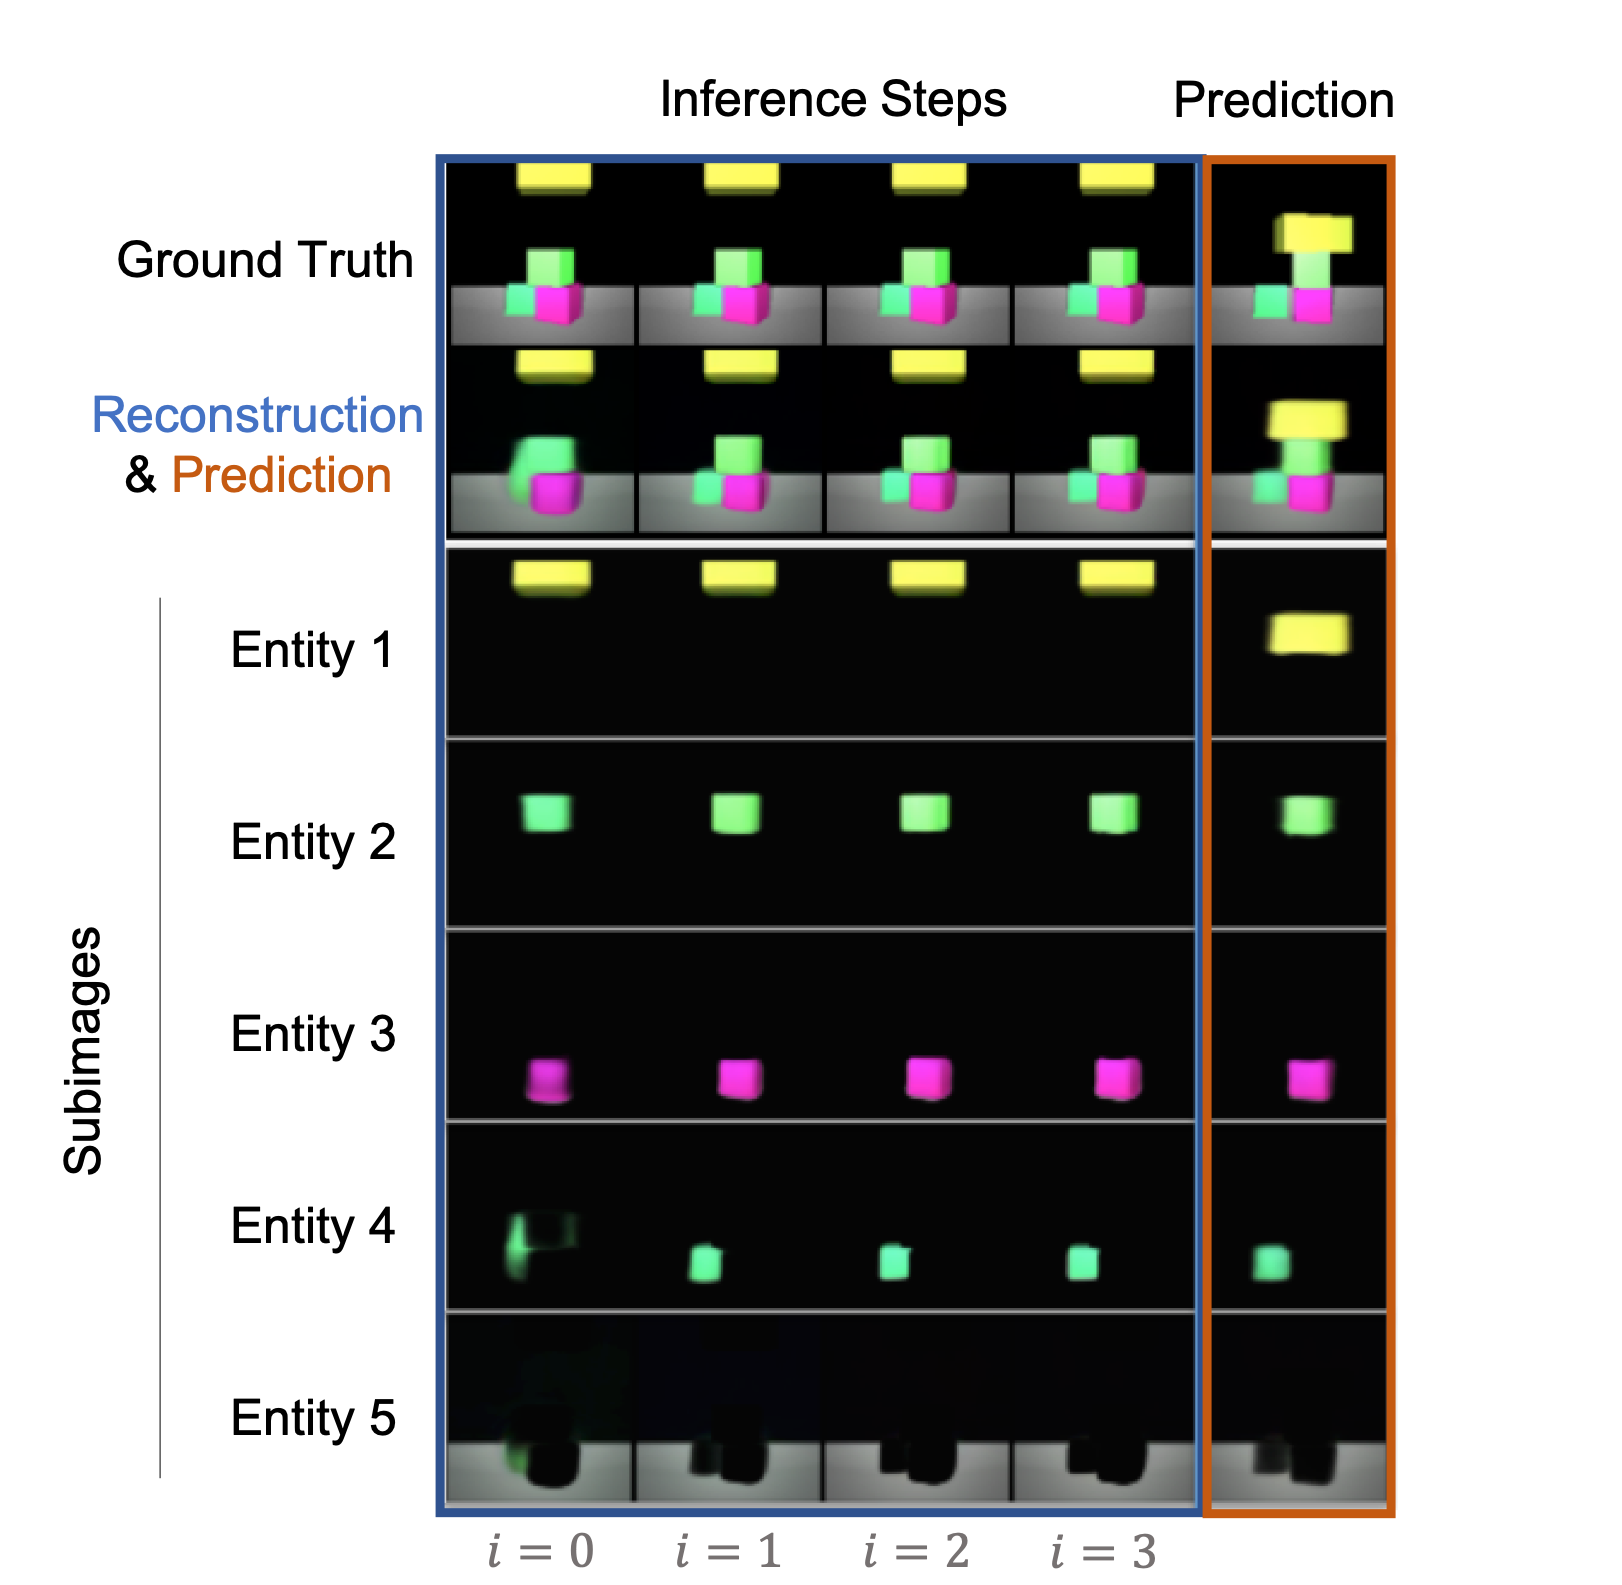
\includegraphics[width=0.5\columnwidth]{figs/experiments/object_segmentation_labeled.png}
    \caption{We show a demonstration of a rollout for the dataset from~\citep{janner2018reasoning}. The first four columns show inference iterations (refinement steps) on the single input image, while the last column shows the predicted results using the dynamics module on the learnt hidden states. The bottom 5 rows show the subimages of each entity at each iteration, demonstrating how the model is able to capture individual objects, and the dynamics afterwards. Notice that OP3 only predicts a change in the yellow block while leaving the other latents unaffected. This is a desriable property for dynamics models that operate on scenes with multiple objects.}
    \label{fig:predicted_components}
\end{figure}

\subsection{Multi-Step Block-Stacking} \label{appdx:multi_step_block_stacking}
The training dataset has 10,000 trajectories each from a separate environment with two different colored blocks. Each trajectory contains five frames (64x64) of randomly picking and placing blocks. We bias the dataset such that 30\% of actions will pick up a block and place it somewhere randomly, 40\% of actions will pick up a block and place it on top of a another random block, and 30\% of actions contain random pick and place locations. Models were trained with K = 4 slots. We optimize actions using CEM but we optimize over multiple consecutive actions into the future executing the sequence with lowest cost. For a goal with $n$ blocks we plan $n$ steps into the future, executing $n$ actions. We repeat this procedure $2n$ times or until the structure is complete. Accuracy is computed as $\frac{\text{\# blocks in correct position}}{\text{\# goal blocks}}$, where a correct position is based on a threshold of the distance error. 
\begin{figure}[h!]
    \centering
    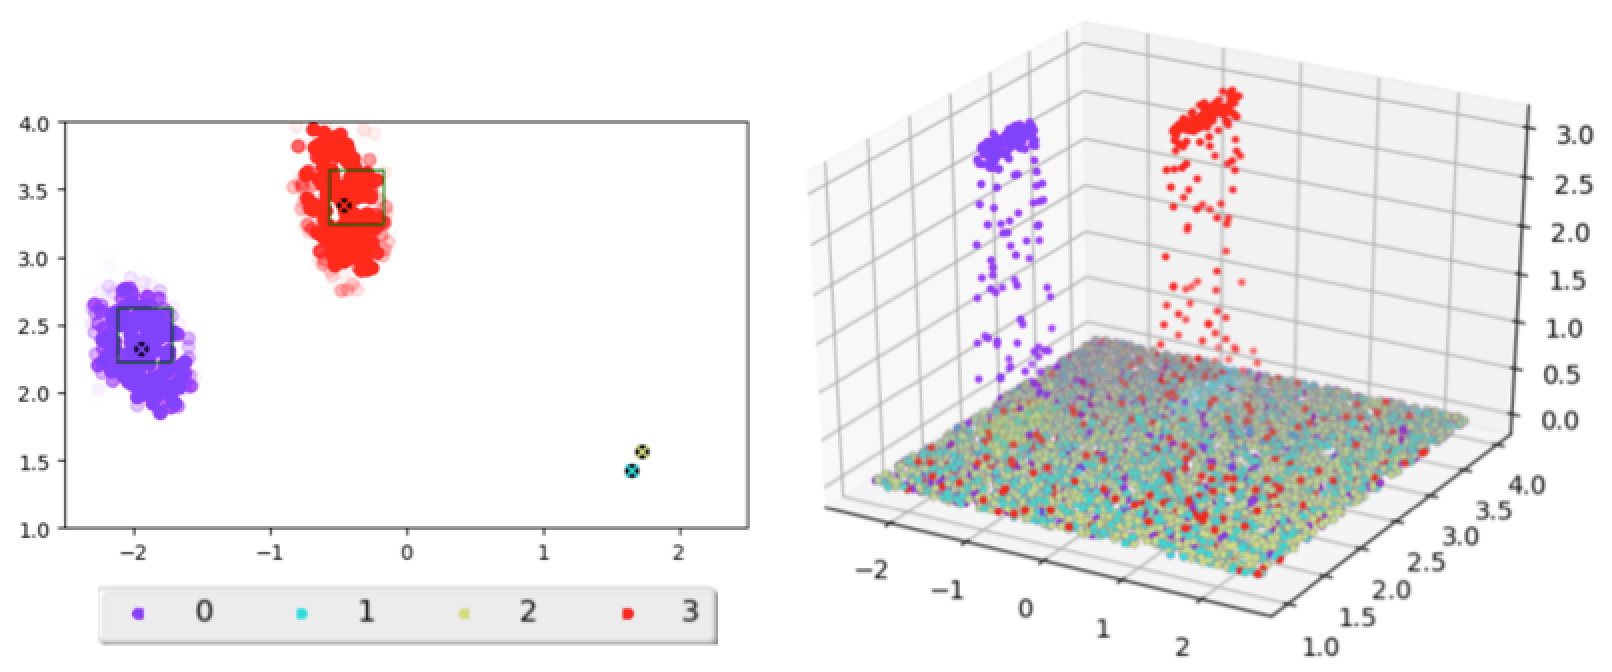
\includegraphics[width=0.8\columnwidth]{figs/experiments/attention_aggregate_v1.png}
    \caption{Two-dimensional (left) and three-dimensional (right) visualization of attention values where colors correspond to different latents. The blocks are shown as the green squares in the 2D visualizatio; picking anywhere within the square automatically picks the block up. The black dots with color crosses denote the computed $\texttt{pick\_xy}$ for a given $h_k$. We see that although the individual values are noisy, the means provide good estimates of valid pick locations. In the right plot we see that attention values for all objects are mostly 0, except in the locations corresponding to the objects (purple and red).}   \label{fig:attention_vizualization}
\end{figure}

For MPC we use two difference action spaces:

\textbf{Coordinate Pick Place:} The normal action space involves choosing a pick (x,y) and place (x,y) location. 

\textbf{Entity Pick Place:} A concern with the normal action space is that successful pick locations are sparse (~2\%) given the current block size. Therefore, the probability of picking $n$ blocks consecutively becomes $0.02^n$ which becomes improbable very fast if we just sample pick locations uniformly. We address this by using the pointers to the entity variables to create an action space that involves directly choosing one of the latent entities to move and then a place $(x,y)$ location. This allows us to easily pick blocks consecutively if we can successfully map a latent \texttt{entity\_id} of a block to a corresponding successful pick location. In order to determine the pick $(x,y)$ from an \texttt{entity\_id} $k$, we sample coordinates uniformly over the pick $(x,y)$ space and then average these coordinates weighted by their attention coefficient on that latent:
$$
\texttt{pick\_xy} | h_k = \frac{\sum_{x',y'} p(h_k|x,y) * \texttt{pick\_x'y'} } {\sum_{x',y'} p(h_k|x',y')}
$$
where $p(h_k|x,y)$ are given by the attention coefficients produced by the dynamics model given $h_k$ and the pick location $(x,y)$ and $x',y'$ are sampled from a uniform distribution.
The attention coefficient of $H_k$ is computed as $\sum_{i\neq k}^K d_{\text{obj-att}}(\tilde{H}_i^{\text{act}}, \tilde{H}_k^{\text{act}})$ (see Appdx.~\ref{appdx:dyn_model})

\section{Ablations}
We perform ablations on the block stacking task from \cite{janner2018reasoning} examining components of our model. Table~\ref{tab:stage1_ablations} shows the effect of non-symmetrical models or cost functions. The ``Unfactorized Model'' and ``No Weight Sharing'' follow (c) and (d) from Figure~\ref{fig:combined_overview} and are unable to sufficiently generalize.
``Unfactorized Cost'' refers to simply taking the mean-squared error of the compositie prediction image and the goal image, rather than decomposing the cost per entity masked subimage.
We see that with the same OP3 model trained on the same data, not using an entity-centric factorization of the cost significantly underperforms a cost function that does decompose the cost per entity (c.f. Table~\ref{tab:mse_results}).
\begin{table}[h]
    \centering
    \begin{tabular}{ccc}
    \toprule
         No Weight Sharing & Unfactorized Model & Unfactorized Cost \\
     \midrule
          0 \% & 0 \% & 5\%\\
    \bottomrule
    \end{tabular}
    \captionof{table}{\small{Accuracy of ablations. The no weight sharing model did not converge during training.}}
    \label{tab:stage1_ablations}
\end{table}

\section{Interpretability}
We do not explicitly explore interpretability in this work, but we see that an entity-factorized model readily lends itself to be interpretable by construction. The ability to decompose a scene into specific latents, view latents invididually, and explicitly see how these latents interact with each other could lead to significantly more interpretable models than current unfactorized models. Our use of attention values to determine the pick locations of blocks scratches the surface of this potential. Additionally, the ability to construct cost functions based off individual latents allows for more interpretable and customizable cost functions.